{\documentclass[11pt,a4paper,titlepage,table]{article}
\usepackage[a4paper]{geometry}
\usepackage[utf8]{inputenc}
\usepackage[english]{babel}
\usepackage{lipsum}

\usepackage{amsmath, amssymb, amsfonts, amsthm, fouriernc}
% mathtools for: Aboxed (put box on last equation in align envirenment)
\usepackage{microtype} %improves the spacing between words and letters

\usepackage{graphicx}
\graphicspath{ {./pics/} {./eps/}}
\usepackage{epsfig}
\usepackage{epstopdf}
\usepackage{colortbl}

%%%%%%%%%%%%%%%%%%%%%%%%%%%%%%%%%%%%%%%%%%%%%%%%%%
%% COLOR DEFINITIONS
%%%%%%%%%%%%%%%%%%%%%%%%%%%%%%%%%%%%%%%%%%%%%%%%%% 
\usepackage{colortbl}
\usepackage[usenames,dvipsnames,svgnames,table]{xcolor}
\usepackage{float}
%%%%%%%%%%%%%%%%%%%%%%%%%%%%%%%%%%%%%%%%%%%%%%%%%%
\definecolor{MyColor1}{HTML}{75A42E}
\definecolor{MyColor2}{HTML}{75A42E}
\definecolor{MyColor3}{HTML}{4D6D1E}
\definecolor{green1}{HTML}{EAF5DB}
\definecolor{green2}{HTML}{C2E193}
\definecolor{maroon}{cmyk}{0,0.87,0.68,0.32}
\newcommand{\textb}{\color{Black} \usefont{OT1}{lmss}{m}{n}}
\newcommand{\blue}{\color{MyColor1} \usefont{OT1}{lmss}{m}{n}}
\newcommand{\blueb}{\color{MyColor1} \usefont{OT1}{lmss}{b}{n}}
\newcommand{\red}{\color{LightCoral} \usefont{OT1}{lmss}{m}{n}}
\newcommand{\green}{\color{Turquoise} \usefont{OT1}{lmss}{m}{n}}
%%%%%%%%%%%%%%%%%%%%%%%%%%%%%%%%%%%%%%%%%%%%%%%%%%

%%%%%%%%%%%%%%%%%%%%%%%%%%%%%%%%%%%%%%%%%%%%%%%%%%
%% FONTS AND COLORS
%%%%%%%%%%%%%%%%%%%%%%%%%%%%%%%%%%%%%%%%%%%%%%%%%%
%    SECTIONS
%%%%%%%%%%%%%%%%%%%%%%%%%%%%%%%%%%%%%%%%%%%%%%%%%%
\usepackage{titlesec}
\usepackage{sectsty}
%%%%%%%%%%%%%%%%%%%%%%%%
%set section/subsections HEADINGS font and color
\sectionfont{\color{MyColor1}}  % sets colour of sections
\subsectionfont{\color{MyColor2}}  % sets colour of sections
\subsubsectionfont{\color{MyColor3}}  % sets colour of sections

%set section enumerator to arabic number (see footnotes markings alternatives)
\renewcommand\thesection{\arabic{section}.} %define sections numbering
\renewcommand\thesubsection{\thesection\arabic{subsection}} %subsec.num.

%define new section style
\newcommand{\mysection}{
	\titleformat{\section} [runin] {\usefont{OT1}{lmss}{b}{n}\color{MyColor1}} 
	{\thesection} {3pt} {} } 

%%%%%%%%%%%%%%%%%%%%%%%%%%%%%%%%%%%%%%%%%%%%%%%%%%
%		CAPTIONS
%%%%%%%%%%%%%%%%%%%%%%%%%%%%%%%%%%%%%%%%%%%%%%%%%%
\usepackage{caption}
\usepackage{subcaption}
%%%%%%%%%%%%%%%%%%%%%%%%
\captionsetup[figure]{labelfont={color=MyColor1}}

\makeatletter
\let\reftagform@=\tagform@
\def\tagform@#1{\maketag@@@{(\ignorespaces\textcolor{red}{#1}\unskip\@@italiccorr)}}
\renewcommand{\eqref}[1]{\textup{\reftagform@{\ref{#1}}}}
\makeatother
\usepackage{hyperref}
\hypersetup{colorlinks=true}

%%%%%%%%%%%%%%%%%%%%%%%%%%%%%%%%%%%%%%%%%%%%%%%%%%
%% PREPARE TITLE
%%%%%%%%%%%%%%%%%%%%%%%%%%%%%%%%%%%%%%%%%%%%%%%%%%
\title{\blue  
	\begin{figure}[h!]
  		\centering
    	\includegraphics[width=1\textwidth]{img/logo3}
	\end{figure}
	\blueb Battle of Origins | Conclusion Chapter}
\author{Patrick Misteli, Ruben Kälin, Jacqueline Staub, Gregory Wyss}
\date{\today}
%%%%%%%%%%%%%%%%%%%%%%%%%%%%%%%%%%%%%%%%%%%%%%%%%%

\begin{document}
	\maketitle
	\hypersetup{linkcolor=MyColor1}	
	
	\tableofcontents
	\newpage
	
	%In this chapter, first provide a summary of your final results including screenshots from your final game. Comment on any significant changes from the alpha release.

	%Next, this chapter should provide commentary about your experience during the class. How well did your initial design ideas materialize into the final game. Were you able to follow your development schedule, or did you deviate significantly from it? How did the different elements of the project structure (development schedule, prototype, playtesting, etc.) contribute to or hinder your progress?

	%Conclude by giving your personal impression of the course. Did it meet your expectations? Are you happy and proud of your game? Do you feel there wasn't enough time or that the schedule was too compressed? You might also consider these questions:

%What was the biggest technical difficulty during the project?
%What was your impression of working with the theme?
%Do you think the theme enhanced your game, or would you have been happier with total freedom?
%What would you do differently in your next game project?
%What was your greatest success during the project?
%Are you happy with the final result of your project?
%Do you consider the project a success?
%To what extend did you meet your project plan and milestones (not at all, partly, mostly, always)?
%What improvements would you suggest for the course organization? (perhaps in D1 evaluation)?
%Did you like the Unity engine?
	
	\section{Current Stage}
	\label{sec:CurrStage}
	
	\subsection{Task Distribution}
	See Table \ref{table:taskallocProject}
	\begin{table}[h!]\centering
		\newcounter{taskId}
		\setcounter{taskId}{0}
		\begin{tabular}{r|p{10cm}|p{1.8cm}|c|c}
			\textbf{Task} & \textbf{Description} & \textbf{Who} & \textbf{Hrs} & \textbf{Actual} \\
			
			\hline 
			\cellcolor[gray]{0.8} & \multicolumn{4}{c}{\cellcolor[gray]{0.8} Idea Finding}\\
			
			\hline				
			\rowcolor{green}		
			\stepcounter{taskId}
			\thetaskId . & Brainstorming Design &\centering  All & $5$ & $7$ \\
			
			\hline
			\rowcolor{green}
			\stepcounter{taskId}
			\thetaskId . & Character modeling &\centering Greg, Jacq  & $20$ & $25$\\
			
			\hline 
			\cellcolor[gray]{0.8} & \multicolumn{4}{c}{\cellcolor[gray]{0.8} Assignments}\\
			
			\hline
			\rowcolor{green}
			\stepcounter{taskId}
			\thetaskId . & Project Proposal Draft & \centering  All & $10$ & $10$\\
			
			\hline
			\rowcolor{green}
			\stepcounter{taskId}
			\thetaskId . & Prototype Chapter& \centering  All & $10$ & $10$\\
			
			\hline
			\rowcolor{green}
			\stepcounter{taskId}
			\thetaskId . & Interim Report Chapter & \centering  All & $10$ & $10$\\
			
			\hline
			\rowcolor{green}
			\stepcounter{taskId}
			\thetaskId . & Alpha Release Chapter & \centering  All & $10$ & $10$\\
			
			\hline
			\rowcolor{green}
			\stepcounter{taskId}
			\thetaskId . & Playtest Chapter & \centering  All & $10$ & $15$\\
			
			\hline
			\rowcolor{green}
			\stepcounter{taskId}
			\thetaskId . & Conclusion Chapter & \centering  All & $10$ & $10$\\
			
			\hline
			\rowcolor{green}
			\stepcounter{taskId}
			\thetaskId . & Demo Video & \centering Patrick & $50$ & $50$\\
			
			\hline 
			\cellcolor[gray]{0.8} & \multicolumn{4}{c}{\cellcolor[gray]{0.8} Presentation and Demos}\\
			
			\hline
			\rowcolor{green}
			\stepcounter{taskId}
			\thetaskId . & Pitch of the Game & \centering  All & $7$ & $7$\\
			
			\hline
			\rowcolor{green}
			\stepcounter{taskId}
			\thetaskId . & Formal Game Proposal & \centering  All & $10$ & $12$\\
			
			\hline
			\rowcolor{green}
			\stepcounter{taskId}
			\thetaskId . & Paper Prototype & \centering  Jacqueline & $5$ & $6$\\
			
			\hline
			\rowcolor{green}
			\stepcounter{taskId}
			\thetaskId . & First Playable Demo & \centering  All & $30$ & $50$\\
			
			\hline
			\rowcolor{green}
			\stepcounter{taskId}
			\thetaskId . & Interim Demo & \centering  All & $50$ & $80$\\
			
			\hline
			\rowcolor{green}
			\stepcounter{taskId}
			\thetaskId . & Alpha Release Demo & \centering  All & $100$ & $50$ \\
			
			\hline
			\rowcolor{green}
			\stepcounter{taskId}
			\thetaskId . & Play-test presentation & \centering  All & $75$ & $100$\\
			
			\hline
			\rowcolor{yellow}
			\stepcounter{taskId}
			\thetaskId . &Final Public Presentation & \centering  All & $40$ & $40$\\
			
							\hline 
				\cellcolor[gray]{0.8} & \multicolumn{4}{c}{\cellcolor[gray]{0.8} Functional Minimum}\\
				
				\hline
				\rowcolor{green}
				\stepcounter{taskId}
				\thetaskId . & Players from two teams running around & \centering  All & $15$ & $15$\\
				
				\hline
				\rowcolor{green}
				\stepcounter{taskId}
				\thetaskId . & Level Design: Overflow flat Map & \centering  All & $15$ & $7$\\
				
				
				\hline
				\rowcolor{green}
				\stepcounter{taskId}
				\thetaskId . & Counting collective hits & \centering  All & $15$ & $8$\\
				
				\hline
				\rowcolor{green}
				\stepcounter{taskId}
				\thetaskId . & Game finishes after 7 min & \centering  All & $15$ &$10$\\
				
				
				\hline
				\rowcolor{green}
				\stepcounter{taskId}
				\thetaskId . & Winner is Team with most hits & \centering  All & $15$ &$14$\\
				
				\hline
				\rowcolor{green}
				\stepcounter{taskId}
				\thetaskId . & AI Controlled Allies/Enemies. & \centering  Ruben & $15$ &$25$\\ 
			
		\end{tabular}
		
		\caption{\textit{Task allocation}  Green: Completed}
		\label{table:taskallocProject}	
	\end{table}	
	
	\newpage
		
		\subsection{Project Management}
		See Table \ref{table:taskallocEngineer}
		\begin{table}[H]\centering
			\begin{tabular}{r|p{10cm}|p{1.8cm}|c|c}
				\textbf{Task} & \textbf{Description} & \textbf{Who} & \textbf{Hrs} & \textbf{Actual} \\
				
				\hline 
				\cellcolor[gray]{0.8} & \multicolumn{4}{c}{\cellcolor[gray]{0.8} Low Target}\\
				
				\hline
				\rowcolor{green}
				\stepcounter{taskId}
				\thetaskId . & Audio: Music + Sound Effects & \centering  Patrick & $15$ & $2$\\
				
				\hline
				\rowcolor{green}
				\stepcounter{taskId}
				\thetaskId . & Physics: Players flying away when hit & \centering  All & $15$ &$10$\\
				
				\hline
				\rowcolor{green}
				\stepcounter{taskId}
				\thetaskId . & Physics: Cooldown before being able to move \& attack & \centering  All & $15$ &$17$\\
				
				\hline
				\rowcolor{green}
				\stepcounter{taskId}
				\thetaskId . & Physics: Immunity cooldown before being vulnerable again & \centering  All & $15$ &$13$\\
				
				\hline
				\rowcolor{green}
				\stepcounter{taskId}
				\thetaskId . & Wonder: Wonder is generated after every 50 collective hits & \centering  All & $15$ &$24$\\
				
				\hline
				\rowcolor{green}
				\stepcounter{taskId}
				\thetaskId . & Wonder: Wonder is (visually) possessed by a human player & \centering  All & $15$ &$10$\\
				
				\hline
				\rowcolor{green}
				\stepcounter{taskId}
				\thetaskId . & Wonder: Wonder can visually be cast & \centering  All & $15$ &$12$\\
				
				
				\hline
				\rowcolor{green}
				\stepcounter{taskId}
				\thetaskId . & Wonder: Wonder converts players & \centering  All & $15$ &$16$\\
				
				\hline
				\rowcolor{green}
				\stepcounter{taskId}
				\thetaskId . & Wonder: Converted Human player plays for the other team & \centering  All & $15$ & $5$\\
				
				
				\hline
				\rowcolor{green}
				\stepcounter{taskId}
				\thetaskId . & Winner is the team with the most members & \centering  All & $15$ &$20$\\
				
				\hline
				\rowcolor{green}
				\stepcounter{taskId}
				\thetaskId . & Level Design: Map includes obstacles & \centering  All & $15$ &$7$\\
				
				\hline 
				\cellcolor[gray]{0.8} & \multicolumn{4}{c}{\cellcolor[gray]{0.8} Desired Target}\\

				\hline
				\rowcolor{green}
				\stepcounter{taskId}
				\thetaskId . & Characters visually polished to look from same theme & \centering Jacqueline, Gregory & $15$ & $150$\\
				
				\hline
				\rowcolor{green}
				\stepcounter{taskId}
				\thetaskId . & Wonder Creation: Creating a wonder by standing together and pressing "commit" & \centering  All & $15$ & $11$\\
				
				\hline
				\rowcolor{green}
				\stepcounter{taskId}
				\thetaskId . & Wonder Creation: Cooldown after releasing "commit" & \centering  All & $15$ & $14$\\
				
				\hline
				\rowcolor{green}
				\stepcounter{taskId}
				\thetaskId . & Wonder Creation: Increased vulnerability during praying & \centering  All & $15$ & $10$\\
				
				\hline
				\rowcolor{green}
				\stepcounter{taskId}
				\thetaskId . & Wonder Creation: Larger praying/studying circles will generate quicker progress & \centering  All & $15$ & $20$\\
				
				\hline
				\rowcolor{green}
				\stepcounter{taskId}
				\thetaskId . & Wonder Creation: AI upgrade to take wonder creation into account & \centering  All & $15$ & $20$\\			
				
				\hline 
				\rowcolor{white}
				\cellcolor[gray]{0.8} & \multicolumn{4}{c}{\cellcolor[gray]{0.8} High Target}\\
				
				\hline
				\rowcolor{green}
				\stepcounter{taskId}
				\thetaskId . & Converted Human player will control free NPC if available & \centering  All & $15$ & $20$\\
				
				\hline
				\rowcolor{green}
				\stepcounter{taskId}
				\thetaskId . & Players evolve numerically according to their actions (Running, Shooting, Praying/Studying) & \centering  All & $15$ & $30$\\
				
				\hline
				\stepcounter{taskId}
				\thetaskId . & Players evolve visually & \centering  All & $15$ &\\
				
				
				\hline 
				\rowcolor{white}
				\cellcolor[gray]{0.8} & \multicolumn{4}{c}{\cellcolor[gray]{0.8} Extras}\\
				
				\hline
				\rowcolor{white}
				\stepcounter{taskId}
				\thetaskId . & Online Multiplayer & \centering  All & $15$ &\\			
				
				\hline
				\rowcolor{white}
				\rowcolor{green}
				\stepcounter{taskId}
				\thetaskId . & Procedural level-design (each level is different)& \centering  All & $15$ & $20$\\		
				
				\hline
				\rowcolor{white}
				\stepcounter{taskId}
				\thetaskId . & Classes of characters (specialized for praying/studying or shooting) & \centering  All & $15$ &\\			
				
				\end{tabular}
				
				\caption{\textit{Task allocation} Green: Completed, Yellow: in Progress}
				\label{table:taskallocEngineer}	
				\end{table}
				
				\newpage
				
				\subsection{Dropped Tasks}
				
				As you can see we did not investigate any further on how to grow body parts, which was originally planned as $task 43$. The reasons for this decision were on the one hand that we encountered several difficulties while working on it and on the other hand that multiple participants of our play-testing sessions inclined to the view that this effect might offend supporters of the religious party. So we decided to ultimately drop this task. Instead we collected feedback by the participants what features they wish for and implemented those instead. You can find a complete list of what extra features we included here:\\
				
				\begin{table}[H]\centering
			\begin{tabular}{r|p{8cm}|p{1.8cm}|c|c}
				\textbf{Task} & \textbf{Description} & \textbf{Who} & \textbf{Hrs} & \textbf{Actual} \\
				
				\hline 
				\cellcolor[gray]{0.8} & \multicolumn{4}{c}{\cellcolor[gray]{0.8} Extended Extras}\\
				
				\hline
				\rowcolor{green}
				\stepcounter{taskId}
				\thetaskId . & Pause menu, with controls & \centering  R, P & $5$ & $5$\\	
				
				\hline
				\rowcolor{green}
				\stepcounter{taskId}
				\thetaskId . & Start menu, players can choose team & \centering  R & $25$ & $25$\\
				
				\hline
				\rowcolor{green}
				\stepcounter{taskId}
				\thetaskId . & End game menu, with statistics & \centering  R, J & $15$ & $15$\\	
				
				\hline
				\rowcolor{green}
				\stepcounter{taskId}
				\thetaskId . & animations for start screen & \centering  J,G & $5$ & $5$\\	
				
				\hline
				\rowcolor{green}
				\stepcounter{taskId}
				\thetaskId . & animations for end game screen & \centering  J, G & $5$ & $5$\\
				
				\hline
				\rowcolor{green}
				\stepcounter{taskId}
				\thetaskId . & Battle Of Origin Soundtrack & \centering  P & $25$ & $25$\\
				
				\hline
				\rowcolor{green}
				\stepcounter{taskId}
				\thetaskId . & Icons for both wonderbars & \centering  J, G & $5$ & $5$\\
				
				\hline
				\rowcolor{green}
				\stepcounter{taskId}
				\thetaskId . & group starts to glow while praying/studying & \centering  G & $10$ & $10$\\
				
				\hline
				\rowcolor{green}
				\stepcounter{taskId}
				\thetaskId . & wonderbar progress indication & \centering  G & $10$ & $10$\\
				
				\hline
				\rowcolor{green}
				\stepcounter{taskId}
				\thetaskId . & wonder collision -> super explosion & \centering  P, R & $25$ & $25$\\
				
				\hline
				\rowcolor{green}
				\stepcounter{taskId}
				\thetaskId . & throwing themed objects instead of power ball & \centering  G, J & $15$ & $15$\\
				
				\hline
				\rowcolor{green}
				\stepcounter{taskId}
				\thetaskId . & allow to push back player with wonder & \centering  G & $5$ & $5$\\
				
				\hline
				\rowcolor{green}
				\stepcounter{taskId}
				\thetaskId . & Indicate wonder duration & \centering  P & $5$ & $5$\\
				\end{tabular}
				
				\caption{\textit{Task allocation} Green: Completed, Yellow: in Progress}
				\label{table:extras}	
				\end{table}
				
				\bigskip
				
				We did some more playtesting sessions after all of these improvements and got a very positive feedback. Since all of the participants filled out the questionnaire already, we did not collect their demographics again, but just let them play the game directly. Afterwards we asked whether they liked the improvements and what they thought they were used for and what they wanted to be different next. The feedback was very positive, which gave us the impression that the changes we made really made a difference.\\  

	\newpage

	
	\section{Some impressions}
	
	Here you can see the final visuals of \textit{Battle Of Origins}: We will start with the presentation of our start screen, where the user gets the opportunity to choose which team he wants to play for. \textit{Battle of Origins} can be played by one to four players. Each of which can fight the battle of Origins either as \textit{Darwinist} or as \textit{Religionist}. Player 1 is responsible to set the number of non-human-players for each team on the start screen (bottom).\\
	
	\begin{figure}[h]
\centering
  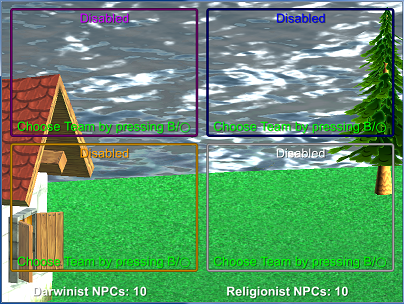
\includegraphics[width=.4\linewidth]{img/startscreen}
  \label{fig:start}
\end{figure}
	
	\begin{figure}[h]
\centering
\begin{minipage}{.5\textwidth}
  \centering
  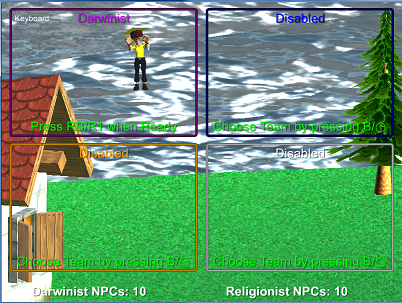
\includegraphics[width=.75\linewidth]{img/startscreenD}
  \label{fig:startD}
\end{minipage}%
\begin{minipage}{.5\textwidth}
  \centering
  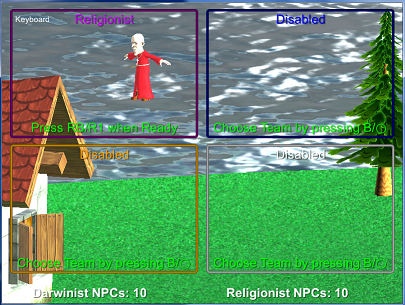
\includegraphics[width=.75\linewidth]{img/startscreenR}
  \label{fig:startR}
\end{minipage}
\end{figure}

The game starts (loading the maps and songs and preparing the game) when all players have chosen their team and committed to them. During this time the players can see how to control their character. A similar menu showing the controls also appears every time some player decides to pause the game by pressing \textit{start}.
	
	\begin{figure}[h]
\centering
  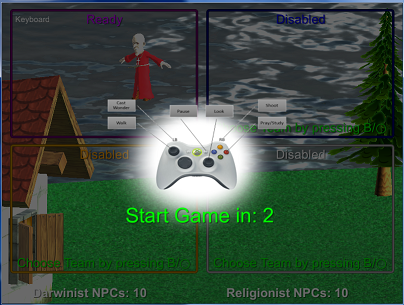
\includegraphics[width=.4\linewidth]{img/uebergangStartGame}
  \label{fig:uebergang}
\end{figure}
	
\newpage

Once the whole map with all obstacles, players and NPC's is loaded as well as all the sounds and the initial scripts are processed, the players can see the map and get some time to find themselves. They can move only after a countdown, displayed by a short \textit{READY?}, \textit{SET}, \textit{GO!}. 	
	
	\begin{figure}[h]
\centering
\begin{minipage}{.3\textwidth}
  \centering
  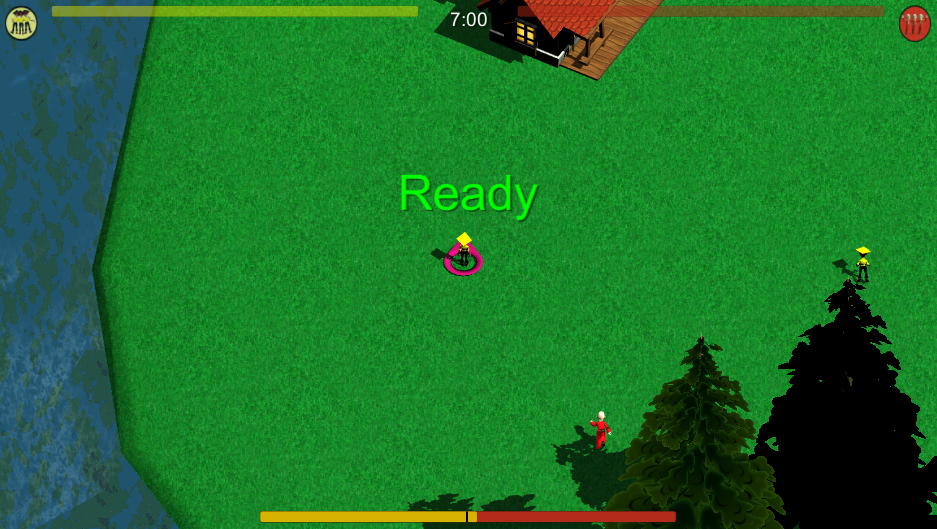
\includegraphics[width=.98\linewidth]{img/countdownReady2}
  \label{fig:ready}
\end{minipage}%
\begin{minipage}{.3\textwidth}
  \centering
  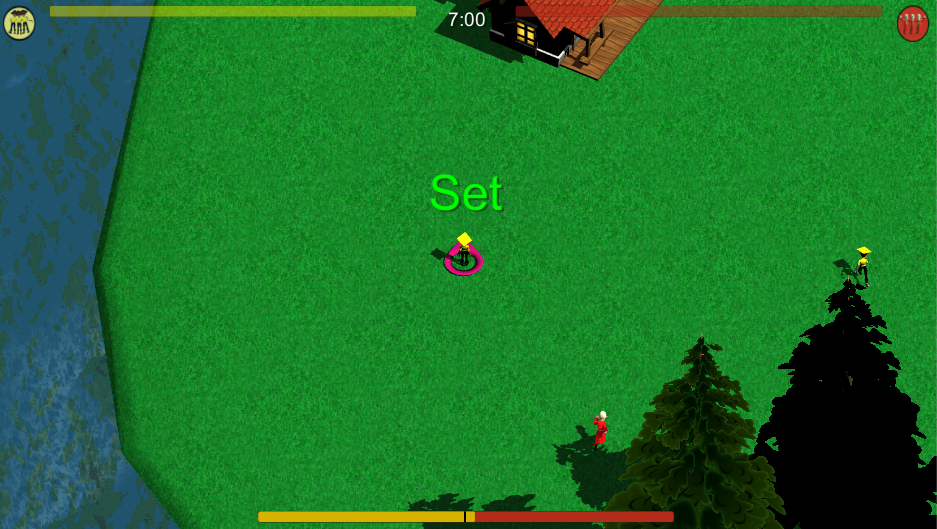
\includegraphics[width=.98\linewidth]{img/countdownSet2}
  \label{fig:set}
\end{minipage}
\begin{minipage}{.3\textwidth}
  \centering
  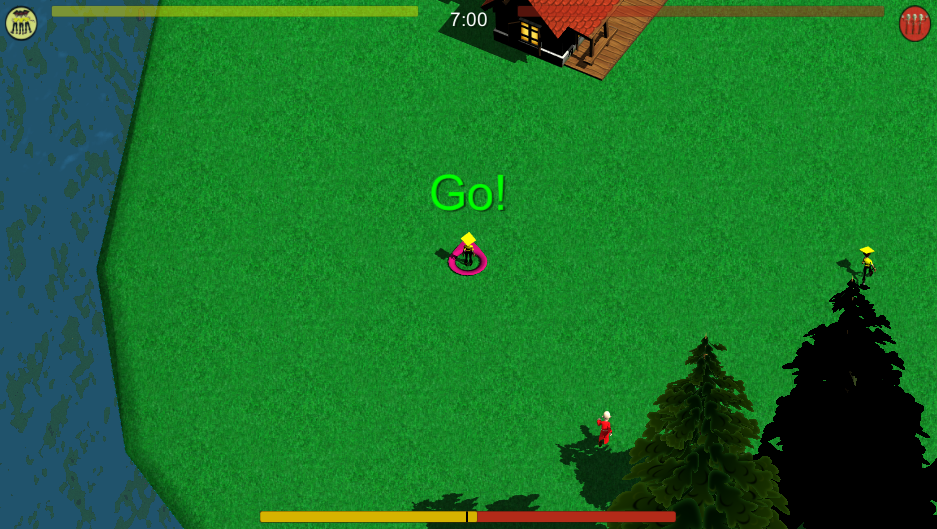
\includegraphics[width=.98\linewidth]{img/countdownGo2}
  \label{fig:go}
\end{minipage}
\end{figure}

The screen holds four graphical user interface elements, to inform the player about important game factors as:
\begin{itemize}
	\item \textbf{Time}: On top of the screen in the middle area a countdown is visible. The game ends either if all characters belong to the same team or after seven minutes.
	\item \textbf{Group Size}: In the bottom of the screen the ratio between members of either team is visible. This information can be used to infer how close either team is to winning the battle.
	\item \textbf{Wonder Bar}: In the top left and right a wonder bar is visible for both teams. This bar gets filled when a group of at least two people is standing together and praying or studying. If the wonder bar is full, a wonder is available for the corresponding team.
\end{itemize}

\bigskip

	\begin{figure}[h]
\centering
  \centering
  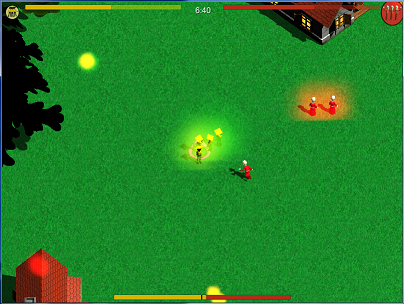
\includegraphics[width=.4\linewidth]{img/PrayIndication}
  \label{fig:prayindication}
\end{figure}

A player can actively make progress and fill up its teams wonder bar by standing together with team mates and praying or studying. While standing together every group is glowing in the corresponding team color (yellow for Darwinists and red for Religionists). They produce small entities of \textit{wonder-energy}, which flows towards their wonder bar on top of the screen.

\newpage

One way to prevent the opponent from reaching their goal (to create a big wonder and converting every character fighting for the other team) is to disperse a group of praying or studying people by shooting at the group. The attacker shoots with an object themed by the corresponding team. Darwinists throw flasks, while Religionists throw crucifixes.

\begin{figure}[h]
\centering
\begin{minipage}{.5\textwidth}
  \centering
  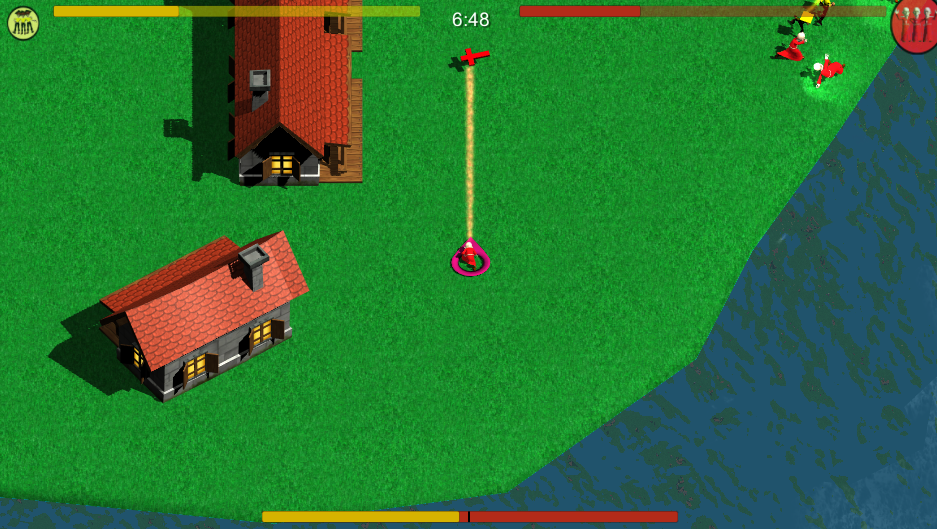
\includegraphics[width=.9\linewidth]{img/ThrowingCross2}
  \label{fig:ThrowingCross}
\end{minipage}%
\begin{minipage}{.5\textwidth}
  \centering
  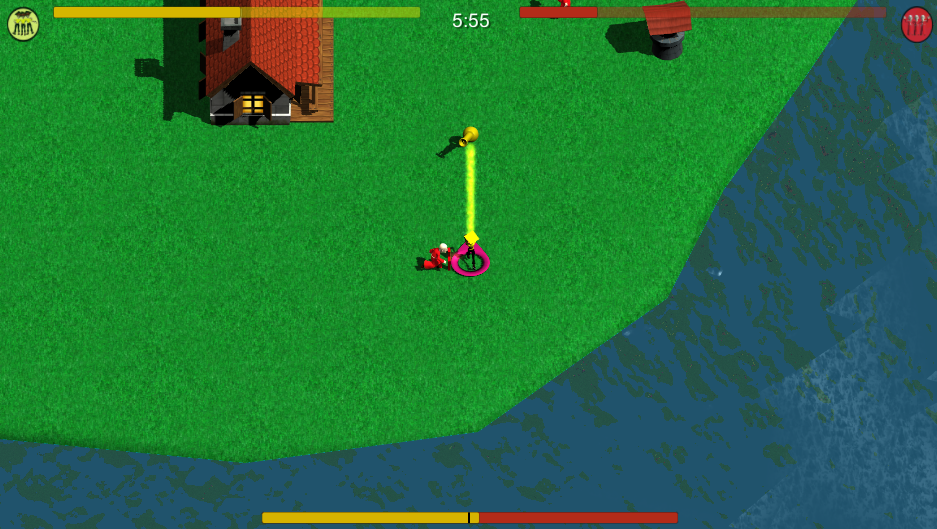
\includegraphics[width=.9\linewidth]{img/ThrowingKolben2}
  \label{fig:ThrowingKolben}
\end{minipage}
\end{figure}

Both teams try to generate a big wonder. Once a wonder bar is full, the corresponding team gets a big wonder. If this team has human team members, the wonder is assigned to one of them. The chosen player can then activate the wonder any time. In teams that consist only of NPCs the wonder is assigned to a random team member and activated instantaneously. Players controlling an activated wonder have the ability to convert enemy players. The wonder lasts for 10 seconds before it expires. The height of the wonder cylinder indicates the remaining duration of the wonder.

	\begin{figure}[h]
  \centering
  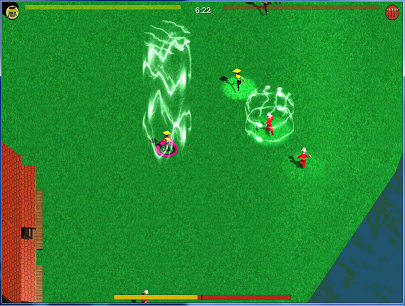
\includegraphics[width=.4\linewidth]{img/wonderdureationIndication}
  \label{fig:wonderdureationIndication}
\end{figure}

If two wonders collide, both wonders get extinguished and a super explosion takes place.

\begin{figure}[h]
  \centering
  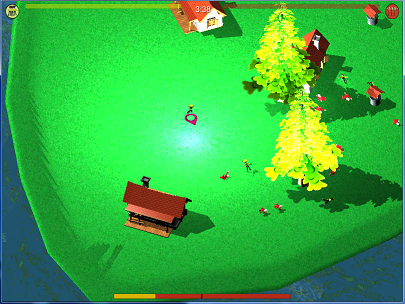
\includegraphics[width=.4\linewidth]{img/wondercollision}
  \label{fig:wondercollision}
\end{figure}

\newpage

\begin{figure}[h]
\centering
\begin{minipage}{.5\textwidth}
  \centering
  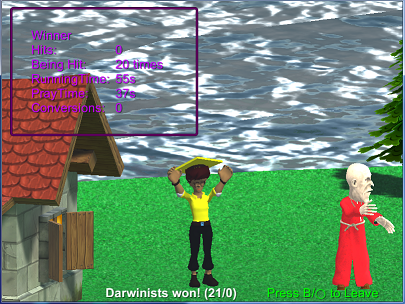
\includegraphics[width=.9\linewidth]{img/winnerD}
  \label{fig:winnerD}
\end{minipage}%
\begin{minipage}{.5\textwidth}
  \centering
  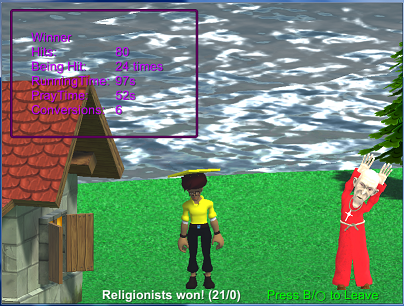
\includegraphics[width=.9\linewidth]{img/winnerR}
  \label{fig:wonderdureationIndication}
\end{minipage}
\end{figure}

The game ends once every player belongs to the same team or seven minutes have passed. In the former case the team who managed to convert every other character wins. In the latter case the team with the most members wins. The end screen displays the winning team as well as some statistics for every player (how often the hit someone, how often they got hit, for how long they were running and praying and how many players they managed to convert).
	
	\section{Feedback}
	
We will answer some specific questions asked by the course organizer:\\

\begin{itemize}
	\item \textbf{How well did your initial design ideas materialize into the final game?}\\
	Very well! We were able to keep almost all the ideas we had when we were working on the paper prototype. Only some small differences, like the perspective did materialize differently than we thought in the beginning.
	
	\item \textbf{Were you able to follow your development schedule?}\\
	To be honest: We did not look too often onto the development schedule. We just met every week and discussed about the problems and possible solutions, what we wanted to work on and where we wanted to be one week later. This worked great for us, since every team member was highly motivated and worked on the project as much as possible.
	
	\newpage
	
	\item \textbf{How did the different elements of the project structure contribute to your progress?}\\
	\textit{game proposal}: We did some brainstorming until we had the topic we wanted to realize in our game, definitively useful!\\
	\textit{paper prototype}: We did not use it to play too often, because it was too slow to be much fun. But it was very useful to think about corner cases we might not have thought about otherwise and proved very useful in anticipating difficulties.\\
	\textit{interim release}: The feedback we got after our presentation was useful, but we had the same thoughts already.\\
	\textit{alpha release}: See interim release...\\
	\textit{playtesting}: This part of the project was extremely useful. We got feedback by more than 60 people in total. We saw which factors caused difficulties and for what kind of people. We tested several settings and investigated on the factors our participants enjoyed the most and on the factors they disliked the most. We collected opinions what they would improve or add and implemented some of those ideas when we were done with our own tasks.  
	
	\item \textbf{Did the course meet your expectations?}\\
	Yes.
	
	\item \textbf{Are you happy with your game?}\\
	Absolutely. If we could start over again, we might take the very same way we already took.\\
	
	\item \textbf{Do you feel there wasn't enough time or that the schedule was too compressed?}\\
	No. In the beginning of the course we were afraid we might not have enough time so we tried to work as productively as possible. But now, in the end, it was enough time to make some silly mistakes, to learn all the unknown platforms and do some tutorials. Especially in the last week we became extremely productive - there is not much left to do now.\\	
	
	\item \textbf{What was the biggest technical difficulty during the project?}\\
	We were surprised that implementing the AI was not the hardest technical difficulty we had. It was more about learning how to interact with maya and blender and how to export the meshes in a way they can be used in unity afterwards. As well as working on the colliders (trying to make them behave exactly the same for both teams).
	
	\item \textbf{What was your impression of working with the theme?}\\
	It was fun. The theme \textit{EVOLUTION} is a very broad topic. It left us with a wide enough field to explore what we wanted to work on. There was no other team going the same way we did, which we appreciated a lot.
	
	\item \textbf{Do you think the theme enhanced your game?}\\
	Sure. No theme at all would have left us with too many options. We enjoyed being restricted by one theme.
	
	\item \textbf{What would you do differently in your next game project?}\\
	Nothing. :-)	
	
	\item \textbf{What was your greatest success during the project?}\\
	Choosing the team. We did very good with our mates. Everybody was eager to work on the topics they chose. We were all interested in slightly different parts, so everybody was able to do what he/she wanted to do. Thus we were productive, motivated and highly encouraged.	
	
	\item \textbf{Are you happy with the final result of your project?}\\
	Of course, our game is great. There is no urge to play \textit{Battle of Origin} ourselves anymore, because we did so A LOT. But it is still fun watching other people playing and enjoying it.
	
	\item \textbf{Do you consider the project a success?}\\
	Yes.	
	
	\item \textbf{To what extend did you meet your project plan and milestones?}\\
	Always.
	
	\item \textbf{What improvements would you suggest for the course organization?}\\
	The presentations were very useful. But the other lectures (especially the ones towards the end of the semester) were not too useful anymore, because we already implemented the thing thought in those lectures. So maybe you could try to invest more time in the beginning of the semester to tell us  everything we might need afterwards and then let the teams work towards the end of the semester, except for the lectures we are supposed to present something.
	
	\item \textbf{Did you like the Unity engine?}\\
	Yes. It takes some time to get into it, but once we knew how it works we started to love it. Even though there are some flaws with Unity, such as the input mapping, that are hopefully improved in the next version, it is still very well suited for this course. 
	
\end{itemize}		
	
	\section{Epilogue}
	
	Thank you so much for the opportunity to work on such a great project. We all are very glad we took the course! Thank you!\\
	
	Sincere,\\
	\textit{Patrick, Ruben, Gregory, Jacqueline}
	
	
\end{document}}{den}
